\documentclass{article}

\usepackage{listings, amssymb, amsmath, tikz-cd, setspace, epigraph, amsthm}

\newtheorem{theorem}{Theorem}[section]

\theoremstyle{definition}
\newtheorem{definition}{Definition}[section]

\usepackage{hyperref}

\usepackage{graphicx}
\graphicspath{ {./images/} }

\hypersetup{pdftex,colorlinks=true,allcolors=blue}
\usepackage{hypcap}

\begin{document}

\title {Contact Geometry}
\maketitle

\centerline{\sc \large The Presentation Notes}
% \vspace{.5pc}
% \vspace{2pc}
\onehalfspace

\tableofcontents

\vspace{2pc}
The latest version of this document can be found at: \url{https://github.com/radicaljims/contact}

\newpage

\textbf{Emphatic note}: none of the mathematical ideas here represent original work in
either content or presentation! The main sources for the material are McInerney
\cite{mcinerney} and Bachman \cite{bachman} but see the full list of references for other very nice resources.

\newpage

\section {Overview}

\epigraph{``Contact geometry is all of geometry.'' VI Arnold.}

Contact Geometry has a history going back centuries and features contributions
from Christiaan Huygens, Sophus Lie and others.

Huygens developed an approach to geometric optics in terms of wavefronts. The way that
wavefronts interact with each other leads to the notion of \textit{contact
  element}. A kind of geodesic flow associated to the space of contact elements
relates Huygen's principle to Fermat's principle of least time and the idea that
light travels along geodesics.

Lie was interested in solutions to differential equations and developed ideas
related to \textit{contact transformations}. The Legendre transformation is a
contact transformation. Contact transformations preserve contact structure.

A unique vector field, the \textit{Reeb field}, can be used to generate families
of contact transformations that can be used to flow contact elements along the field.

Physics appears to still be a central source of insight and applications -
especially to thermodynamics and the Hamiltonian formulation of classical mechanics.

This small text and accompanying presentation will mostly focus on a few of the
underlying geometric ideas, excluding contact transformations almost entirely.

Here's what we'll be talking about:

\begin{itemize}
\item contact elements
\item fields of planes and a bit about foliations
\item differential forms and the contact one-form
\item the non-integrability condition
\item the Reeb field associated to a contact one-form
\end {itemize}


\section {Contact Elements}

A contact element to a manifold is a hyperplane at a point of the manifold. For
all of these notes and the presentation this manifold will be $\mathbb{R}^{2}$
or $\mathbb{R}^{3}$ or subsets thereof.

Let's work in the plane $\mathbb{R}^{2}$ for a moment. Then a contact element is a point $p
\in \mathbb{R}^{2}$ and a non-vertical line-segment centered at $p$. We could
call a collection of these at every point of $\mathbb{R}^{2}$ a field of line-segments.

We need three parameters to describe this space, which we will denote
$\mathbb{CR}^{2} = \{ (x, y, m) | x, y, m \in \mathbb{R} \}$.

The $(x, y)$ components correspond to the points in the plane and the $m$
represents the slope of the line through that point.

In a little bit we will be interested in picking out certain subsets of this
space and spaces like this.

(To visualize this one can imagine a pin-wheel of planar segments, orthogonal to
$\mathbb{R}^{2}$, sitting in $\mathbb{R}^{3}$ ``above'' $\mathbb{R}^{2}$.)

\subsection {Foliations and Integrability}

If we imagine a sequence of points as being sampled from a regular curve, and the line-segments
the associated tangents, then we could integrate the tangents to recover the curve.

Usually we think of differentiating curves to get tangents, not integrating them
to get curves! Continuing in this kind of reverse direction we might call the curve an
\textit{integral curve}. I think we have seen such things a few times in class when
talking about extending some local piece of a curve on a patch to the entire surface.

If we bump up a dimension and imagine a field of planes we are led to consider
integrating those planes into an \textit{integral surface}.

Integral curves and surfaces are examples of foliations. They decompose a space
into a disjoint union of subspaces and seem pretty cool! And they certainly seem
like a cool thing to make with our contact elements!

But here's the punch line - the fields of planes we talk about in contact
geometry are \textbf{maximally} non-integrable!

This non-integrability is ensured by a condition on the gadget we use to
character our plane fields - the contact one form.

\section {Differential Forms}

Differential forms give us a way to talk about directed linear subspaces. In
particular we can use a one-form (the so-called \textbf{contact one-form}) to
characterize fields contact elements.

\subsection{Covectors and the Dual Space}
We've talked about at least three different forms in class: the first, second,
and third fundamental forms.

They are called \textit{forms} because they are functions that map vectors to a
number. The fundamental forms are also \textit{bilinear}, but there are also simpler
\textit{linear} forms. We will call these \textbf{one-forms}.

If you've taken enough linear algebra you may recognize one-forms as living in
the \textit{dual space} $\mathbb{V}^{*}$ associated to a vector space
$\mathbb{V}$. If you've taken enough physics you may recognize these as \textit{covectors}.

From a geometrical perspective a very important fact about covectors is that
they have a natural pairing with vectors. If $v \in \mathbb{V}$ and $w \in \mathbb{V}^{*}$ then the number $w(v) \in
\mathbb{R}$ is \textbf{invariant}: it does not depend on what basis $v$ or $w$
may be expressed in.

Said another way the pairing does not depend on coordinates!

Avoiding coordinate representations as much as possible is a big goal of this
formalism. Nonetheless I am about to introduce bases for both $\mathbb{V}$ and $\mathbb{V}^{*}$!

For a given basis $e_{i}$ of $\mathbb{V}$ there is an associated basis $e^{j}$
of $\mathbb{V}^{*}$ called the \textbf{dual basis}.

The dual basis has the property that under the pairing we have $e^{j}(e_{i}) = \delta^{j}_{i}$.

That is the \textbf{Kronecker delta} which is $1$ when $i = j$ and $0$
otherwise.

If we then write a $v \in \mathbb{R}^{2}$ as $v = ae_{1} + be_{2}$ and apply the
dual form $e^{1}$ we get:

\begin{align*}
  e^{1} (v) = \\
  e^{1}(ae_{1} + be_{2}) = \\
  e^{1}(ae_{1}) + e^{1}(be_{2}) = \\
  a(e^{1}(e_{1})) + b(e^{1}(e_{2})) = \\
  a * 1 + b * 0 = \\
  a
\end{align*}

This shows that elements of the dual basis are projection functions.

If we specialize to the context of differential geometry then our $\mathbb{V}$
becomes a tangent plane or space, maybe $T_{p}\mathbb{R}^{3}$. The dual vector space $\mathbb{V}^{*}$ then becomes the \textbf{cotangent space}
denoted $T_{p}^{*}\mathbb{R}^{3}$.

Remember these are just linear functions that
map tangent vectors to real numbers!

In class we're used to writing $\rho_{u}, \rho_{v}$ or maybe $r_{u}, r_{v}$ as a
basis for the tanget space.

In these notes we're going to try to use $\frac{\partial}{\partial x}, \frac{\partial}{\partial
  y}, \frac{\partial}{\partial z}$ for the tangent space and $dx, dy, dz$ for the cotangent space.

\subsection{One-forms, Two-forms, Three-forms}

Differential forms are grounded in \textit{multilinear} algebra, so we'll be
interested in \textit{multilinear} functions. But a very specific kind of
multilinear function - antisymmetric (or sometimes skew-symmetric) ones.

We actually already know an antisymmetric multilinear function and that is the
cross product!

That's going to be handy because one way to motivate the idea of (not yet
differential) forms is to try to generalize the cross product to higher
dimensions.

It turns out you can't, exactly, but you can get something even cooler: the
\textbf{wedge} (or exterior) product.

Why is it cooler? It exists for every dimension and it lets you build linear
subspaces of arbitrary rank in the same way that a cross product kind of
represents a plane.

In fact the cross product of two vectors in $\mathbb{R}^{3}$
is dual in a sense to the wedge product of two vectors. The cross product being
the normal associated to the plane while the wedge product represents the subset
of the plane spanned by the parallelogram formed by the vectors.

Before we go any further we want to emphasize that in this section we are
usually only working with covectors but the wedge product can operate on general
vector spaces. The point is, it makes sense to take the exterior product of any sort of vector, not just the
ones that hang out in tangent or cotangent spaces.

However since we do care mostly about dual spaces, I'll tell you that if you take
the wedge product of two one-forms you get a \textbf{two-form}. We'll look at a
calculation in a second, but in words a two-form is an antisymmetric bilinear
form.

That means it's a bilinear map $w: \mathbb{V} \times \mathbb{V} \to \mathbb{R}$
that satisfies $w(a, b) = -w(b, a)$.

Secretly you already know an antisymmetric bilinear form: the 2 x 2 determinant!
And in fact this is what we'll use to define the wedge product.

So, given two one forms $v, w$ we want to create a two-form that will map two
vectors $a, b$ to a real number. The recipe goes like this:

$
(v \wedge w) (a, b) =
\begin{vmatrix}
  v (a) & w (a) \\
  v (b) & w (b)
\end{vmatrix}
$

An interesting consequence is that $v \wedge v = 0$ for every one-form $v$.

I should also emphasize that the antisymmetry gives the wedge product an
orientation! So these are oriented linear subspaces!

Let's have an example. Given two two-forms $w = 2dx - 3dy + dz$ and $v = dx +
2dy - dz$ and two vectors $a = \frac{\partial}{\partial x} +
3\frac{\partial}{\partial y} + \frac{\partial}{\partial z}$ and $b =
2\frac{\partial}{\partial x} - \frac{\partial}{\partial y} +
3\frac{\partial}{\partial z}$ we can compute their wedge product as:

\begin{align*}
  \begin{vmatrix}
    w (a) & v(a) \\
    w (b) & v(b)
  \end{vmatrix} =
  \begin{vmatrix}
    (2 - 9 + 1) & (1 + 6 - 1) \\
    (4 + 3 + 3) & (2 - 2 -3)
  \end{vmatrix} =
  \begin{vmatrix}
    -6 & 6 \\
    10 & -3 
  \end{vmatrix} = 18 - 60 = -42
\end{align*}

We can keep going and given three one-forms build the three-form

$
(u \wedge v \wedge \wedge w) (a, b, c) =
\begin{vmatrix}
  u (a) & v (a) & w (a) \\
  u (b) & v (b) & w (b) \\
  u (c) & v (c) & w (c) \\
\end{vmatrix}
$

for arbitrary vectors $a, b, c$.

We can keep building forms of higher degree if we keep going up a dimension but
we're going to stop here and summarize what we have.

These are:

\begin{itemize}
  \item three one-forms $dx, dy, dz$ that act on vectors $a, b, c$
  \item three two-forms $dx \wedge dy, dy \wedge dz, dz \wedge dx$ that act on
    pairs of vectors $(a, b)$
  \item one three form $dx \wedge dy \wedge dz$ that act on triples of vectors
    $(a, b, c)$
\end{itemize}

And collectively we will call these \textit{k-forms}.

In the same way that we can let a vector's coefficients vary and get a vector
field we can also let the coefficients of a k-form vary and
it is \textit{this} that we call a \textbf{differential form}.

So a differential two-form looks like $u = f dx \wedge dy$ where f is a
differential function.

\subsection {Exterior differentiation}

I won't keep you in suspense any longer! \textit{Yes}, there is a way to
differentiate a differential form!

It behaves a lot like the usual derivative, as we'll see shortly, and also has
the curious effect of bumping up the degree of a k-form. So the derivative of a
zero-form is a one-form, of a one-form is a two-form, and so on.

Oh did I talk about zero-forms before? Then now's a good time to say that a
zero-form is just a smooth function $f : \mathbb{R}^{N} \to \mathbb{R}$.

Now we can say what we want the \textbf{exterior derivative} to do to the
various forms.

\begin{itemize}
  \item on a zero-form $f$ we have the usual derivative, $df$, which is
    now a one-form that maps a tangent vector to a number
  \item on a one-form $u = f dx$ we have the two-form $du = df \wedge dx$
  \item on a two-form $v = f dx \wedge dy$ we have the three-form $dv = df \wedge dx \wedge
    dy$
  \item on a three-form we have $dw = df \wedge dx \wedge dy \wedge dz$ but
    we don't want four-forms so pretend this never happened
\end{itemize}

The exterior derivative is linear and satisfies a kind of Leibniz rule:

\begin{gather*}
  d(cv) = c * dv \\
  d(v + w) = dv + dw \\
  d(v \wedge w) = dv \wedge w + (-1)^{pq} v \wedge dw
\end{gather*}

where $p$ is the \textit{degree} (0, 1, 2, 3) of $v$ and $q$ the degree of $w$.

A \textit{very} import property: $d^{2} = 0$. This is related to the notion of
cohomology and is maybe fundamental to all physics! At least people on the
Internet will whisper that.

Differentiating forms can quickly get out of hand but for smaller ones it isn't
too bad. Let's see what the derivative of $v = ydx + xdy$ is.

\begin{align*}
  dv = \\
  d(ydx + xdy) = \\
  d(ydx) + d(xdy) = \\
  dy \wedge dx + dx \wedge dy = \\
  -dx \wedge dy + dx \wedge dy = \\
  0
\end{align*}

Now that we know about differential forms and the exterior derivative we can
talk about contact forms!

\subsection {Contact Forms}

Note: most of what we describe below is with respect to general vector spaces.
It still applies when working now with the space of all contact elements in $C\mathbb{R}^{2}$ or
$C\mathbb{R}^{3}$! 

A one-form determines a field of planes through it's \textbf{kernel}: the set of
vectors it maps to zero.

A plane in $\mathbb{R}^{3}$ is the set of vectors satisfying $Ax + By + Cz = 0$.
Remembering that the dual basis $dx, dy, dz$ are projection functions we can see
this is equivalent to the one-form $Adx + Bdy + Cdz = 0$.

For a one-form $v$ to be a \textbf{contact one-form} it must also satisfy this
non-degeneracy condition:

\begin{equation}
  dv \wedge v \neq = 0
\end{equation}

The non-degeneracy condition on the contact form ensures that corresponding
field of planes will be \textit{non-integrable}, as we rather mysteriously
desire.

Real quick while I have you, are you wondering if there's a condition on the
one-form that ensures \textit{integrability}?

There is! The result is called \textbf{Frobenius' theorem} (I think there might
be a couple of those) and it says that the field of planes is integrable when

\begin{equation}
  dv \wedge v = 0
\end{equation}

So people like to say that in fact contact one-forms are \textit{maximally non-integrable}!

Okay, remember $\mathbb{CR}^{2}$? It's the space of contact elements for
$\mathbb{R}^2$. We claim that it can be represented by the one-form $dy - mdx$.

Let's check the non-degeneracy condition.

\begin{align*}
  d (dy - mdx) \wedge (dy - mdx) = \\
  -dm \wedge dx \wedge (dy - mdx) = \\
  -dm \wedge dx \wedge dy = \\
  -dx \wedge dy \wedge dm
\end{align*}

Which is the \textit{volume} form for $\mathbb{CR}^{2}$ and is non-zero.

We can also try to understand what the kernel of $w = dy - mdx$ looks like by seeing
how the form acts on a vector $x = a\frac{\partial}{\partial x} +
b\frac{\partial}{\partial y} + c\frac{\partial}{\partial z}$ when they pair to 0.

\begin{align*}
  w (x) = \\
  (dy - mdx) (a\frac{\partial}{\partial x} +
  b\frac{\partial}{\partial y} + c\frac{\partial}{\partial z}) = \\
  (dy)(a\frac{\partial}{\partial x} +
b\frac{\partial}{\partial y} + c\frac{\partial}{\partial z}) - (mdx)(a\frac{\partial}{\partial x} +
b\frac{\partial}{\partial y} + c\frac{\partial}{\partial z}) = \\
  b - ma = 0
\end{align*}

It's interesting to note that this says our slope $m$ is the ratio of the $y$
and $x$ components of our vector field.

Substituting $b = ma$ into our equation for $x$ we can find a basis for the
kernel of $w$.

\begin{align*}
  a\frac{\partial}{\partial x} +
    b\frac{\partial}{\partial y} + c\frac{\partial}{\partial z}) = \\
  a\frac{\partial}{\partial x} +
    ma\frac{\partial}{\partial y} + c\frac{\partial}{\partial z}) = \\
  a(\frac{\partial}{\partial x} +
    m\frac{\partial}{\partial y}) + c\frac{\partial}{\partial z}) 
\end{align*}

So $\ker(w) = span(\frac{\partial}{\partial x} +
    m\frac{\partial}{\partial y}, \frac{\partial}{\partial z})$ which will be a
two-dimensional subspace of the three-dimensional $\mathbb{CR}^{2}$ as we would hope!

The standard contact form for $\mathbb{R}^{3}$ is $xdy + dz$. We can check this
is a contact form:

\begin{align*}
  d (xdy + dz) \wedge (xdy + dz) = \\
  (dx \wedge dy + d^{2} z) \wedge (xdx + dz) = \\
  (dx \wedge dy) \wedge (xdy + dz) = \\
  (dx \wedge dy \wedge xdy) + (dx \wedge dy \wedge dz) = \\
  dx \wedge dy \wedge dz
\end{align*}

It is important to note that a given contact form does not \textit{uniquely}
determine a plane field. We can ``multiply'' $v$ by a function $f$ without
changing the kernel.

There is also a theorem of Darboux that says locally all contact forms have
``the same'' structure.

So the differences between contact structures only start to show up at the
\textit{global} level. That might make the non-integrability condition
especially interesting since we can't ``just integrate'' the contact form to understand
the global structure of the plane field!

But just because two contact forms have the same kernel \textit{doesn't} mean
they have the same Reeb field, our next and findal topic!

\section {Reeb field}

All the pieces (plane distributions, contact one-forms, contact transformations)
seem to come together with Reeb fields, but I haven't much to say on them.

A Reeb field $R$ for a contact one-form $w$ is the unique vector field that satisfies the following constraints:

\begin{gather*}
  R \in \ker(dw) \\
  w(R) = 1
\end{gather*}
  
If we move (flow) our contact elements along a Reeb field then we get another
non-integrable set of contact elements. Somewhat akin to parallel transporting a
vector along a parallel vector field?

\section {Theorems and Definitions}

Here we list some precise theorems and definitions. See \cite{mcinerney} for additional details.

\theoremstyle{definition}
\begin{definition} A \textit{contact element} in $\mathbb{R}^{2}$ is a pair $(P,
  l)$ consisting of a point $P \in \mathbb{R}^{2}$ and a nonvertical line $l
  \subset \mathbb{R}^{2}$ such that $P \in l$. The set of all contact elements
  in $\mathbb{R}^{2}$ is denoted $C\mathbb{R}^{2}$.
\end{definition}

There is a standard system of coordinates for $C\mathbb{R}^{2}$: $\{(x, y, m) |
  x, y, m \in \mathbb{R}^{2}\}$. Note that $C\mathbb{R}^{2}$ is isomorphic to $\mathbb{R}^{3}$.

\begin{definition} A \textit{contact form} on $\mathbb{R}^{3}$ is a one-form
  $\alpha$ on $\mathbb{R}^{3}$ that is non-degenerate: for all $p \in
  \mathbb{R}^{3}$, $\alpha_{p} \wedge d\alpha_{p} \neq 0$. The \textit{contact
    distribution} $E_{\alpha}$ associated to $\alpha$ is the plane field defined
  by $E_{\alpha} = \ker \alpha$.
\end{definition}

The standard contact form on $\mathbb{R}^{3}$ is $\alpha_{0} = xdy + dz$ which is
non-degenerate since $\alpha_{0} \wedge d\alpha_{0} = dx \wedge dy \wedge dz$.

The following is a theorem of \textbf{Frobenius}.

\begin{theorem} 
Let $E$ be a $k$-dimensional distribution in $\mathbb{R}^{n}$ with the property
that for all $p \in \mathbb{R}^{n}$ and $X_{p}, Y_{p} \in E_{p}$, we have
$[X_{o}, Y_{p}] \in E_{p}$ (closure under Lie brackets). Then $E$ is locally
integrable in the following sense: for each $p \in \mathbb{R}^{n}$, there exists
a domain $U_{p} \subset \mathbb{R}^{k}$ and a smooth regular parametrization
$\phi : U_{p} \to \mathbb{R}^{n}$ such that $p \in S = \phi(U_{p})$ and such
that for all $q \in S, E_{q} = T_{q}S$. Moreover, there exist a domain $V_{p}
\subset \mathbb{R}^{n}$ containing $p$ and a smooth function $F : V_{p} \to
\mathbb{R}^{n - k}$ such that $S \cap V_{p} = F^{-1}(0)$.

Conversely, if $E$ is integrable then for all $p \in R^{n}$ and all vector
fields $X, Y$ such that $X_{p}, Y_{p} \in E_{p}$ for all $p \in \mathbb{R}^{n}$,
$[X_{p}, Y_{p}] \in E_{p}$.
\end{theorem}

\begin{theorem} Let $E$ be a plane field in $\mathbb{R}^{3}$ defined as the
  kernel of a one-form $\alpha$ so that $E = \ker \alpha$. Then $E$ is
  integrable if and only if $\alpha \wedge d\alpha = 0$.
\end{theorem}

\begin{theorem} Let $\alpha$ be a contact form on $\mathbb{R}^{3}$. There is a
  unique vector field $\chi$ with the properties that
  \begin{itemize}
    \item $\alpha(\chi) = 1$
    \item $i(\chi)d\alpha = 0$
  \end{itemize}

  where $i$ is the interior product. The vector field $\chi$ is called the \textit{Reeb field} of $\alpha$.
\end{theorem}

\begin{theorem} Let $\alpha$ be a contact form on $\mathbb{R}^{3}$ with
  corresponding Reeb field $\chi$ and contact distribution $E$. Then every
  smooth vector field $X$ on $\mathbb{R}^{3}$ can be written uniquely as
  \begin{equation*}
    X = f(\chi) + H(X)
  \end{equation*}
  where $f : \mathbb{R}^{3} \to \mathbb{R}$ is a smooth function and $H(X)$ is a
  smooth vector field such that for all $p \in \mathbb{R}^{3}, H_{p}(X) \in E_{p}$.
\end{theorem}

Here is \textbf{Darboux's theorem for contact geometry}. 

\begin{theorem} Let $(\mathbb{R}^{3}, \alpha)$ be a contact space and let
  $\alpha_{0} = xdy + dz$ be the stanard contact from on $\mathbb{R}^{3}$. For
  all $p \in \mathbb{R}^{3}$ there are a domain $U$ containing $p$ and a
  diffeomorphism $\phi : U \to \phi(U) \subset \mathbb{R}^{3}$ such that
  $\phi(p) = p$ and such that $\phi^{*}\alpha = \alpha_{0}$ on $U$.
\end{theorem}

\newpage

\section {Questions and Feedback}

Have any questions? I can try to answer them in subsequent versions!

See any errors or omissions? Please let me know!

\newpage

\section {Pictures}

\subsection {Contact Elements}

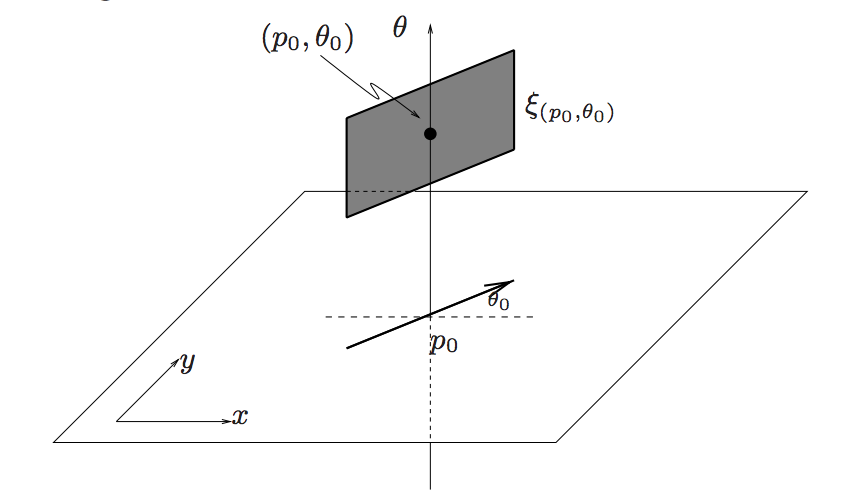
\includegraphics[scale=0.8]{geiges_contact_structure}

The contact structure for $C\mathbb{R}^{2}$ aka $dy - mdx$ from \cite{geiges}.

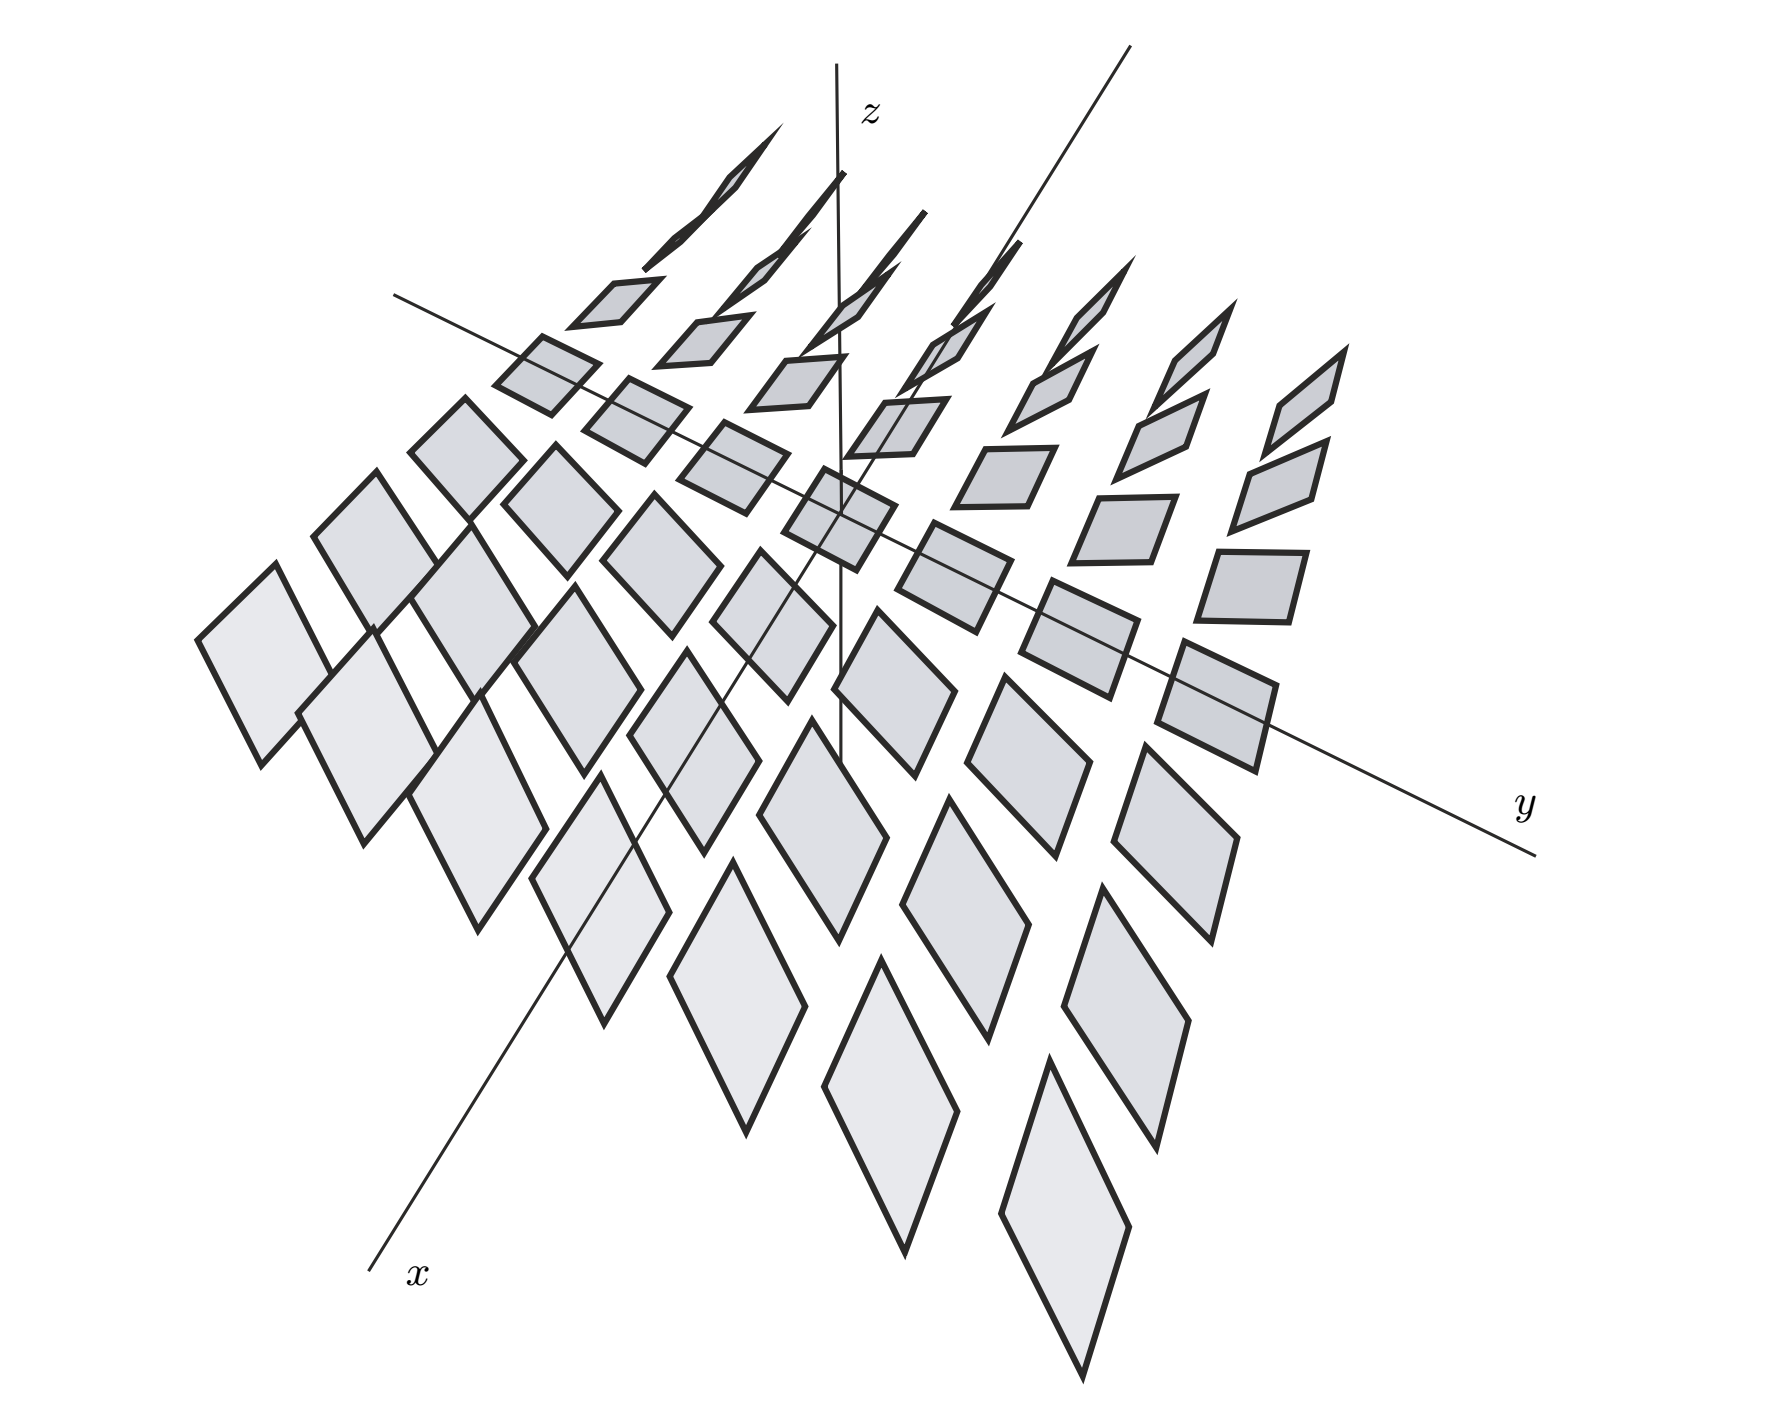
\includegraphics[scale=0.3]{contact_elements_bachman}

The contact structure generated by $xdy + dz$ from \cite{bachman}.

\subsection {Visualizing forms}

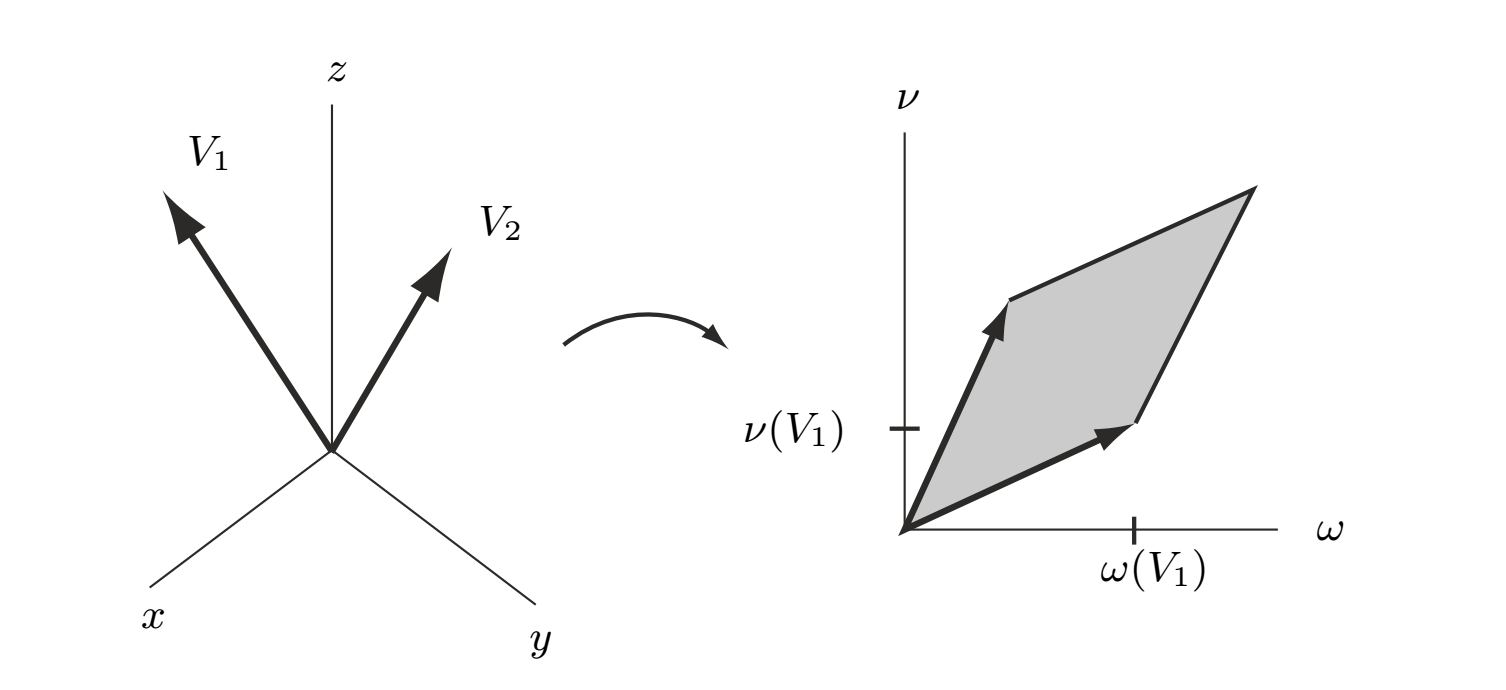
\includegraphics[scale=0.5]{form_vis_bachman}

Visualizing 2-forms from \cite{bachman}.


\begin{thebibliography}{9}

\phantomsection
\addcontentsline{toc}{section}{References}
  
\bibitem{mcinerney} 
  Andrew McInerney
  \textit{First Steps in Differential Geometry: Riemannian, Contact, Symplectic}. 
  Springer-Verlag New York, 2013.

\bibitem{bachman}
  David Bachman
  \textit{A Geometric Approach to Differential Forms}.
  Birkhäuser Basel, 2006.

\bibitem{toponogov} 
  Victor Andreevich Toponogov
  \textit{Differential Geometry of Curves and Surfaces: A Concise Guide}. 
  Birkhäuser, 2006

\bibitem{geiges}
  Hansjörg Geiges
  \textit{Christiaan Huygens and contact geometry}
  eprint arXiv:math/0501255

\end{thebibliography}



\end{document}